% ============================================================
%   CVE Text-Property-Graph example sub-graph + security pass
%   For: "Buffer overflow in OpenSSL 1.0.1f"
% ============================================================
%
% Companion to CVE-graph-example.tex. Same linguistic backbone
% (SENTENCE, TOKENs, NOUN_PHRASE, ENTITY) drawn in the base
% colours, plus the security frontend overlay: three new
% security-entity nodes (VULN_TYPE, SOFTWARE, VERSION) connected
% to the underlying TOKEN nodes with dashed red edges. The
% TOKEN row is extended by one cell so the version literal
% "1.0.1f" has its own TOKEN to attach to.
%
% Page sized close to the figure bounding box for two-column
% inclusion: 
\includegraphics[width=\linewidth]{CVE-graph-example-security}.
%
% Compile:
%   pdflatex -interaction=nonstopmode CVE-graph-example-security.tex
% ============================================================

\documentclass[10pt]{article}

\usepackage[paperwidth=215mm, paperheight=180mm, margin=4mm]{geometry}
\usepackage{tikz}
\usepackage{amsmath}
\usepackage{amssymb}
\pagestyle{empty}

\usetikzlibrary{positioning, arrows.meta, calc, fit, backgrounds}

% -- Colour palette (matches model_architecture.tex) --
\definecolor{nodeBase}{RGB}{ 70,130,180}
\definecolor{nodeSec}{RGB}{200, 80, 80}
\definecolor{edgeBase}{RGB}{ 60, 60, 60}
\definecolor{edgeSec}{RGB}{160, 50, 50}
\definecolor{accent}{RGB}{ 20, 70,140}
\definecolor{frameFill}{RGB}{249,250,252}

\tikzset{
    bignode/.style={
        rounded corners=2pt, draw=nodeBase, fill=white,
        line width=0.45pt, inner sep=3pt,
        font=\scriptsize\sffamily, minimum height=5mm,
    },
    secnode/.style={
        rounded corners=2pt, draw=nodeSec, fill=white,
        line width=0.5pt, inner sep=3pt,
        font=\scriptsize\sffamily, minimum height=5mm,
    },
    rootnode/.style={
        rounded corners=2pt, draw=accent, fill=white,
        line width=0.6pt, inner sep=3pt,
        font=\scriptsize\sffamily\bfseries, minimum height=5mm,
    },
    lin/.style={
        -{Stealth[length=2mm]}, line width=0.45pt, draw=edgeBase,
    },
    seclin/.style={
        -{Stealth[length=2mm]}, line width=0.5pt, draw=edgeSec, dashed,
    },
    elab/.style={
        font=\tiny\sffamily, text=edgeBase,
        inner sep=1pt,
        fill=white, fill opacity=0.92, text opacity=1,
        rounded corners=1pt,
    },
    seclab/.style={
        font=\tiny\sffamily, text=edgeSec,
        inner sep=1pt,
        fill=white, fill opacity=0.92, text opacity=1,
        rounded corners=1pt,
    },
    title/.style={
        font=\sffamily\bfseries\small, text=accent,
    },
    subtitle/.style={
        font=\sffamily\scriptsize, text=black!65,
    },
    legbox/.style={
        rectangle, rounded corners=1.5pt, draw=black!40, fill=white,
        line width=0.3pt, inner sep=3pt, font=\tiny\sffamily,
        align=left,
    },
}

\begin{document}

\noindent
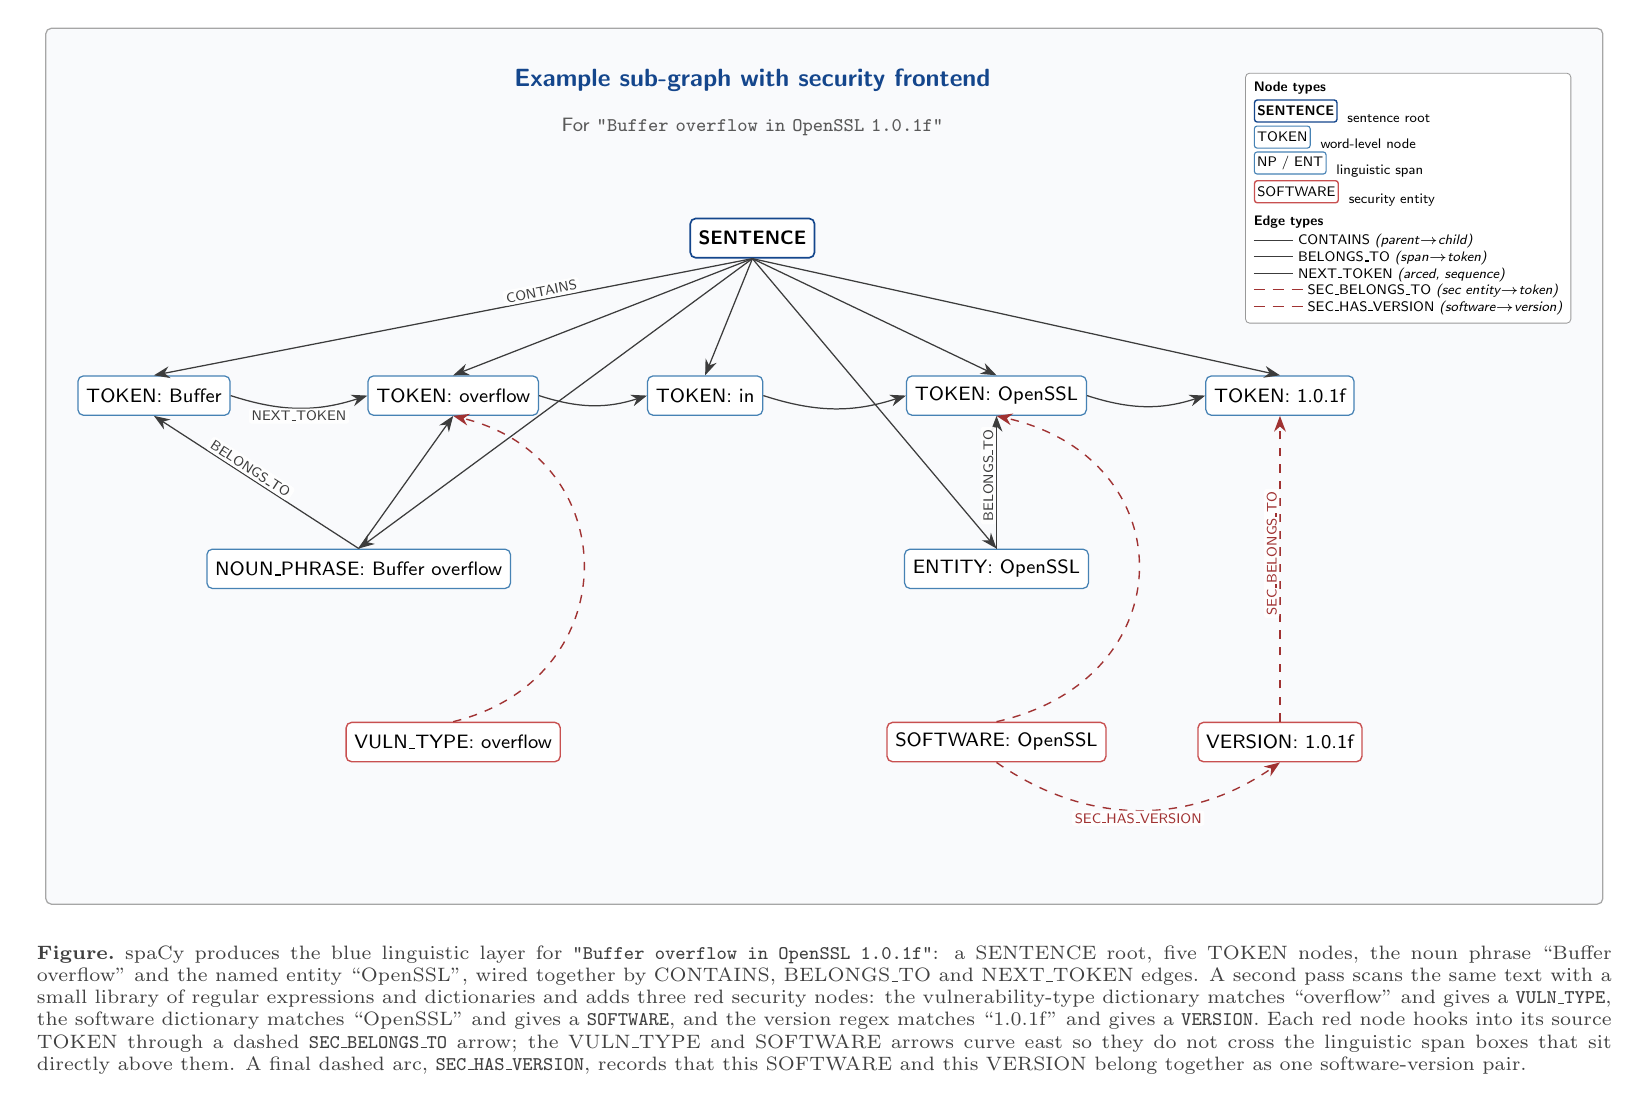
\begin{tikzpicture}

% ============================================================
%   Title block
% ============================================================
\node[title] (ttl) at (0, 6.0) {Example sub-graph with security frontend};
\node[subtitle, below=0.8mm of ttl, text width=115mm, align=center] (sub)
    {For \texttt{"Buffer overflow in OpenSSL 1.0.1f"}};

% ============================================================
%   Base linguistic nodes
% ============================================================
\node[rootnode] (S)  at ( 0.0,  4.0) {SENTENCE};

% Five TOKEN cells: now including the version literal.
\node[bignode] (T1) at (-7.6,  2.0) {TOKEN: Buffer};
\node[bignode] (T2) at (-3.8,  2.0) {TOKEN: overflow};
\node[bignode] (T3) at (-0.6,  2.0) {TOKEN: in};
\node[bignode] (T4) at ( 3.1,  2.0) {TOKEN: OpenSSL};
\node[bignode] (T5) at ( 6.7,  2.0) {TOKEN: 1.0.1f};

\node[bignode] (NP) at (-5.0, -0.2) {NOUN\_PHRASE: Buffer overflow};
\node[bignode] (E)  at ( 3.1, -0.2) {ENTITY: OpenSSL};

% ============================================================
%   Security-frontend nodes (red overlay)
% ============================================================
\node[secnode] (VT) at (-3.8, -2.4) {VULN\_TYPE: overflow};
\node[secnode] (SW) at ( 3.1, -2.4) {SOFTWARE: OpenSSL};
\node[secnode] (VR) at ( 6.7, -2.4) {VERSION: 1.0.1f};

% ============================================================
%   Base edges (gray solid)
%   - SENTENCE -> {T1..T5, NP, E}             [CONTAINS]
%   - NP -> {T1, T2}, ENTITY -> T4            [BELONGS_TO]
%   - T1 -> T2 -> T3 -> T4 -> T5              [NEXT_TOKEN, arced]
% ============================================================

% CONTAINS
\draw[lin] (S.south) --
    node[elab, pos=0.35, sloped, above=0pt] {CONTAINS} (T1.north);
\draw[lin] (S.south) -- (T2.north);
\draw[lin] (S.south) -- (T3.north);
\draw[lin] (S.south) -- (T4.north);
\draw[lin] (S.south) -- (T5.north);
\draw[lin] (S.south) -- (NP.north);
\draw[lin] (S.south) -- (E.north);

% BELONGS_TO
\draw[lin] (NP.north) --
    node[elab, pos=0.55, sloped, above=0pt] {BELONGS\_TO} (T1.south);
\draw[lin] (NP.north) -- (T2.south);
\draw[lin] (E.north)  --
    node[elab, pos=0.55, sloped, above=0pt] {BELONGS\_TO} (T4.south);

% NEXT_TOKEN (one labelled, the rest implicit)
\draw[lin] (T1.east) to[bend right=18]
    node[elab, midway, below=0pt] {NEXT\_TOKEN} (T2.west);
\draw[lin] (T2.east) to[bend right=18] (T3.west);
\draw[lin] (T3.east) to[bend right=18] (T4.west);
\draw[lin] (T4.east) to[bend right=18] (T5.west);

% ============================================================
%   Security-pass edges (red dashed)
%   Each security entity attaches to the TOKEN whose surface
%   form the regex / dictionary matched.
%
%   VT and T2 share x = -3.8, and SW and T4 share x = 3.1, so a
%   straight vertical sec->token line would pierce NP (which
%   spans x in [-6.75, -3.25]) or ENTITY (x in [2.0, 4.2]).
%
%   Earlier the file used `to[bend right=...]' for these two
%   edges, but the rendered arcs did not bulge far enough east
%   to clear ENTITY (TikZ's bend angle controls endpoint
%   tangents, not the sag we want). We now route them as
%   Bezier curves with two east-of-obstacle control points,
%   which gives precise lateral clearance:
%     - VT -> T2 controls pull the curve to x = -1.6 at
%       mid-height (NP.east = -3.25, clearance 1.65 cm).
%     - SW -> T4 controls pull the curve to x = 5.5 at
%       mid-height (ENTITY.east = 4.2, clearance 1.3 cm).
%   VR -> T5 has no obstacle and stays straight, so we put the
%   single SEC_BELONGS_TO label on it.
% ============================================================
\draw[seclin] (VT.north) .. controls (-1.6, -1.6) and (-1.6,  1.2) .. (T2.south);
\draw[seclin] (SW.north) .. controls ( 5.5, -1.6) and ( 5.5,  1.2) .. (T4.south);
\draw[seclin] (VR.north) --
    node[seclab, pos=0.55, sloped, above=0pt] {SEC\_BELONGS\_TO} (T5.south);

% Software -> Version pairing (intra-security relation), drawn
% as a downward arc so the label has room below the secnode row
% (the straight gap between SW.east and VR.west is only ~1 cm).
% arcfloor coordinate is added to the frame fit list so the
% outer frame fully encloses the arc.
\coordinate (arcfloor) at ($(SW.south)!0.5!(VR.south)+(0,-1.4cm)$);
\draw[seclin] (SW.south) to[bend right=35]
    node[seclab, midway, below=0pt] {SEC\_HAS\_VERSION} (VR.south);

% ============================================================
%   Legend (top-right): node + edge key
% ============================================================
\node[legbox, anchor=north east] (leg) at (10.4, 6.1) {
    \textbf{Node types}\\[1pt]
    \tikz{\node[draw=accent, fill=white, line width=0.5pt,
                rounded corners=1pt, font=\tiny\sffamily\bfseries,
                minimum height=2.8mm, inner sep=1pt] {SENTENCE};}\ \
        sentence root\\
    \tikz{\node[draw=nodeBase, fill=white, line width=0.4pt,
                rounded corners=1pt, font=\tiny\sffamily,
                minimum height=2.8mm, inner sep=1pt] {TOKEN};}\ \
        word-level node\\
    \tikz{\node[draw=nodeBase, fill=white, line width=0.4pt,
                rounded corners=1pt, font=\tiny\sffamily,
                minimum height=2.8mm, inner sep=1pt] {NP / ENT};}\ \
        linguistic span\\
    \tikz{\node[draw=nodeSec, fill=white, line width=0.5pt,
                rounded corners=1pt, font=\tiny\sffamily,
                minimum height=2.8mm, inner sep=1pt] {SOFTWARE};}\ \
        security entity\\[2pt]
    \textbf{Edge types}\\[1pt]
    \textcolor{edgeBase}{\rule[0.55mm]{5mm}{0.4pt}}\ CONTAINS\
        \textit{(parent$\to$child)}\\
    \textcolor{edgeBase}{\rule[0.55mm]{5mm}{0.4pt}}\ BELONGS\_TO\
        \textit{(span$\to$token)}\\
    \textcolor{edgeBase}{\rule[0.55mm]{5mm}{0.4pt}}\ NEXT\_TOKEN\
        \textit{(arced, sequence)}\\
    \textcolor{edgeSec}{\rule[0.55mm]{1.4mm}{0.4pt}\rule[0.55mm]{1.0mm}{0pt}\rule[0.55mm]{1.4mm}{0.4pt}\rule[0.55mm]{1.0mm}{0pt}\rule[0.55mm]{1.4mm}{0.4pt}}\ SEC\_BELONGS\_TO\
        \textit{(sec entity$\to$token)}\\
    \textcolor{edgeSec}{\rule[0.55mm]{1.4mm}{0.4pt}\rule[0.55mm]{1.0mm}{0pt}\rule[0.55mm]{1.4mm}{0.4pt}\rule[0.55mm]{1.0mm}{0pt}\rule[0.55mm]{1.4mm}{0.4pt}}\ SEC\_HAS\_VERSION\
        \textit{(software$\to$version)}
};

% ============================================================
%   Outer frame
% ============================================================
\begin{scope}[on background layer]
    \node[draw=black!35, line width=0.45pt, rounded corners=2pt,
          fill=frameFill,
          fit=(ttl)(sub)(S)(T1)(T5)(NP)(E)(VT)(SW)(VR)(arcfloor)(leg),
          inner sep=4mm] (frame) {};
\end{scope}

% ============================================================
%   Caption (below the frame). Kept inside the standalone
%   bounding box so the figure is self-contained when viewed
%   on its own. When the figure is included in a paper via
%   \includegraphics{}, prefer the suggested \caption{...}
%   block reproduced as a comment at the end of this file.
% ============================================================
\node[font=\scriptsize, text=black!75, text width=200mm,
      align=justify, below=4mm of frame.south, anchor=north]
      (cap) {%
    \textbf{Figure.}\  spaCy produces the blue
    linguistic layer for
    \texttt{"Buffer overflow in OpenSSL 1.0.1f"}: a SENTENCE
    root, five TOKEN nodes, the noun phrase ``Buffer
    overflow'' and the named entity ``OpenSSL'', wired
    together by CONTAINS, BELONGS\_TO and NEXT\_TOKEN edges.
    A second pass scans the same text with a small library
    of regular expressions and dictionaries and adds three
    red security nodes: the vulnerability-type dictionary
    matches ``overflow'' and gives a \texttt{VULN\_TYPE}, the
    software dictionary matches ``OpenSSL'' and gives a
    \texttt{SOFTWARE}, and the version regex matches
    ``1.0.1f'' and gives a \texttt{VERSION}. Each red node
    hooks into its source TOKEN through a dashed
    \texttt{SEC\_BELONGS\_TO} arrow; the VULN\_TYPE and
    SOFTWARE arrows curve east so they do not cross the
    linguistic span boxes that sit directly above them. A
    final dashed arc, \texttt{SEC\_HAS\_VERSION}, records
    that this SOFTWARE and this VERSION belong together as
    one software-version pair.
};

\end{tikzpicture}

\end{document}

% ============================================================
%   Suggested LaTeX caption for paper integration
% ============================================================
%
% Copy this into a \begin{figure*}...\end{figure*} block:
%
% \begin{figure*}[t]
%   \centering
%   
\includegraphics[width=\linewidth]{CVE-graph-example-security}
%   \caption{The same TPG slice with the security frontend
%   layered on top. spaCy produces the blue linguistic layer
%   for \texttt{"Buffer overflow in OpenSSL 1.0.1f"} (one
%   SENTENCE root, five TOKEN nodes, the noun phrase
%   ``Buffer overflow'' and the named entity ``OpenSSL''),
%   connected by CONTAINS, BELONGS\_TO and NEXT\_TOKEN edges.
%   A second pass scans the same text with a small library
%   of regular expressions and dictionaries and adds three
%   red security nodes: VULN\_TYPE for ``overflow'',
%   SOFTWARE for ``OpenSSL'' and VERSION for ``1.0.1f''.
%   Each red node hooks into its source TOKEN through a
%   dashed SEC\_BELONGS\_TO arrow, and the dashed
%   SEC\_HAS\_VERSION arc records that this SOFTWARE and
%   this VERSION belong together as one software-version
%   pair.}
%   \label{fig:cve-graph-example-security}
% \end{figure*}
%
% ============================================================
